\documentclass[paper=a4, fontsize=11pt, ngerman, abstract=on]{scrartcl}

\usepackage{tocloft}
\usepackage{titling}
\usepackage{blindtext}
\usepackage[utf8]{inputenc}
\usepackage[T1]{fontenc}
\usepackage[ngerman]{babel}
\usepackage{amsmath,amsfonts,amsthm}
\usepackage{siunitx}
\sisetup{output-decimal-marker = {,}}
\usepackage{graphicx}

\usepackage{sectsty}
\allsectionsfont{\raggedright \normalfont\scshape}

\usepackage{fancyhdr}
\pagestyle{fancyplain}

\fancyhead{} % Head Footer
\fancyfoot[L]{} % Left Footer
\fancyfoot[C]{} % Center Footer
\fancyfoot[R]{\thepage} % Right Footer - Page numbering
\renewcommand{\headrulewidth}{0pt} % Remove header underlines
\renewcommand{\footrulewidth}{0pt} % Remove footer underlines
\setlength{\headheight}{13.6pt} % Customize the height of the header

\numberwithin{equation}{section} % Number equations within sections (i.e. 1.1, 1.2, 2.1, 2.2 instead of 1, 2, 3, 4)
\numberwithin{figure}{section} % Number figures within sections (i.e. 1.1, 1.2, 2.1, 2.2 instead of 1, 2, 3, 4)
\numberwithin{table}{section} % Number tables within sections (i.e. 1.1, 1.2, 2.1, 2.2 instead of 1, 2, 3, 4)

\setlength\parindent{0pt} % Removes all indentation from paragraphs - comment this line for an assignment with lots of text

\newcommand {\horrule}[1]{\rule{\linewidth}{#1}} % Create horizontal rule command with 1 argument of height

\usepackage{listings}
\usepackage{color} %red, green, blue, yellow, cyan, magenta, black, white
\definecolor{mygreen}{RGB}{28,172,0} % color values Red, Green, Blue
\definecolor{mylilas}{RGB}{170,55,241}
\lstdefinestyle{matlab}{language=Matlab,%
  breaklines=true,%
  morekeywords={matlab2tikz},
  keywordstyle=\color{blue},%
  morekeywords=[2]{1}, keywordstyle=[2]{\color{black}},
  identifierstyle=\color{black},%
  stringstyle=\color{mylilas},
  commentstyle=\color{mygreen},%
  showstringspaces=false,%without this there will be a symbol in the places where there is a space
  basicstyle=\footnotesize,
  stepnumber=1,
  emph=[1]{for,end,break},emphstyle=[1]\color{blue},
  frame=tb,
  rulesepcolor=\color{gray},
  rulecolor=\color{gray},
  framesep=3pt,
  xleftmargin=3pt,
  xrightmargin=8pt,
  tabsize=2,
}

\begin{document}

\title {
  \normalfont \normalsize
  \textsc{HAW Hamburg} \\ [25pt]
  \textsc{Modellierung Dynamischer Systeme} \\ [15pt]
  \horrule{0.5pt} \\[0.4cm] % Thin top horizontal rule
  \huge Ausbreitung von Tuberkulose \\ [15pt] % The assignment title
  \small Ein Populationsmodell \\ [15pt]
  \small Prof. Dr. Fohl \\
  \horrule{1pt} \\[0.5cm] % Thick bottom horizontal rule
}

\author{
  Matthias Nitsche \\
  \texttt{matthias.nitsche@haw-hamburg.de} \\
  \small{Hamburg University of Applied Sciences, Department of Computer Science} \\
  \small{Berliner Tor 7} \\
  \small{20099 Hamburg, Germany} \\
}

\begin{document}

\maketitle

\renewcaptionname{ngerman}{\abstractname}{Kurzfassung}
\begin{abstract}
In dieser Arbeit wird eine Übersicht von mathematischen Analyseverfahren zur Übertragung von Tuberkulose präsentiert. Hierzu zählen die Compartment Modelle wie SEIR und agentenbasierte Modelle (ABM). Tuberkulose ist eine komplexe Erkrankung mit unterschiedlichen Krankheitsstadien. Das Ziel von derartigen Modellierungen ist das identifizieren von optimalen Parametern, sodass ein teil der Realität dargestellt werden kann. Dies führt idealerweise zu neuen Erkenntnissen wie z.B. durch Impfung Tuberkulose langfristig verhindert werden kann. Auf dem Weg wird der Einfluss von Impfung, Immunerkrankungen, Alter und Lokalität untersucht. Modelle dieser Arbeit wurden mit hilfe von Matlab und Python Mesa realisiert.
\end{abstract}

\newpage

\renewcommand{\cftsecleader}{\cftdotfill{\cftdotsep}}
\tableofcontents

\newpage

% \begin{figure}[ht]
%   \centering
%   \includegraphics[width=\linewidth,height=8cm,keepaspectratio]{images/test}
%   \caption{My caption}
%   \label{fig:test-label}
% \end{figure}

\section{Domäne - Tuberkulose}

Tuberkulose ist eine bakterielle Infektionserkrankung die besonders häufig die Lunge befällt. Die WHO schätzt Tuberkulose als eine der top 10 Todesursachen der Welt, mit einer Sterberate von 1.8 Millionen Menschen und 10.4 Millionen Neuinfektionen in 2015. Es ist ein aktives Sustainable Development Goal (SDG) das bis 2030 eingedämpft werden soll. Tuberkulose ist eine Krankheit die in Ländern mit schlechter medizinischer Versorgung und tropischem Klima (Sonne und starker Regen) gesondert auftritt. \cite{WHOTB2016}

\subsection{Krankheitsbild}

Tuberkulose (TB) wird vor allem über die Luft übertragen. Das befallen der Lungen resultiert nicht zwangsweise in einer aktiven Infektion der Krankheit. In Abbildung \ref{fig:tuberculosis-cycle} ist der Kreislauf der Tuberkulose Übertragung.

\begin{figure}[ht]
  \centering
  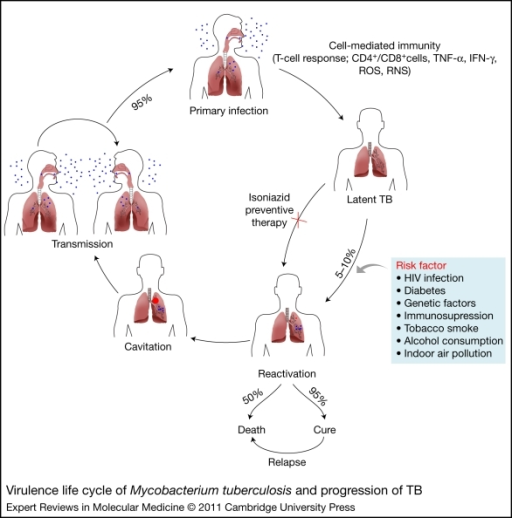
\includegraphics[width=0.5\textwidth,keepaspectratio]{images/tuberculosis-cycle}
  \caption{Tuberkulose Kreislauf in \cite{Kumar2011}}
  \label{fig:tuberculosis-cycle}
\end{figure}

In kurz, ein Mensch wird über direkten Kontakt von einem anderen über die Luft mit Tuberkulose latent infiziert, hat wesentlich geringere Chancen infiziert zu werden und eine hohe Chance bei nicht Medikation zu sterben.

\begin{enumerate}
  \item{Die \textbf{Übertragung} findet über die Luft zwischen zwei Menschen statt. Häufig ist deshalb der Ort der Übertragung in Lebensgemeinschaften auf engem Raum, öffentlichen Verkehrsmitteln oder Arbeitsplätzen. Klimaanlagen beschleunigen die Verbreitung von Bakterien in der Luft. Bei direktem Kontakt ist die Chance auf Ansteckung bei 95\% und es wird eine hauptinfektion ausgelöst.}
  \item{Die \textbf{Hauptinfektion} ist meist ein befallen der Lunge. Verschiedene Immunfaktoren beeinflussen die Geschwindigkeit des Fortschreitens.}
  \item{Betroffene sind ab diesem Schritt \textbf{latent infiziert}. Während das Subjekt in der latenten TB Phase ist tauchen nicht zwangsweise Symptome auf. Die meisten latent infizierten Träger von TB haben in ihrem ganzen Leben keinerlei Auswirkungen der Krankheit. In dem latenten Stadium können Subjekte niemanden anstecken. Einige Faktoren beeinflussen jedoch die Wahrscheinlichkeit auf eine aktive Infektion, sogenannte Risikofaktoren. Diese sind vor allem Immunbedingt wie z.B. HIV, Diabetes, genetische Faktoren, Immunsupressiver und viele mehr. Subjekte mit derartigen Ausprägungen haben eine Wahrscheinlichkeit von 5-10\% die Krankheit als aktive Infektion zu tragen. In den Fällen wo eine Präventivtherapie nicht hilft erfolgt meist eine aktive Krankheitsentwicklung.}
  \item{Die \textbf{aktive Infektion/Reaktivierung} erfolgt irgendwann nachdem ein Subjekt latent infiziert wurde. Ab diesem Punkt gibt es nur zwei Möglichkeiten, Menschen die eine Heilung bekommen werden zu 95\% wieder gesund. 50\% die keine Heilung bekommen sterben und 50\% bessern sich von selbst. Ein Rückfall führt meistens zum Tode. Infizierte sind ab jetzt Überträger der Krankheit. Menschen die von TB geheilt werden gehen zurück ins latente Stadium. Eine vollständige Heilung ist nicht mehr möglich.}
\end{enumerate}

An diesem Model wird relativ schnell klar warum TB so gefährlich ist. Betroffene können nie wieder von der Krankheit regenerieren und Immunfaktoren, die besonders im Alter schlechter werden begünstigen den Ausbruch der Krankheit. Zudem kommt das TB in zwei Formen auftritt. TB als herkömliche, behandelbare Erkrankung und Multi-Drug-Resistant TB (MDR-TB), bei der TB ressistent gegenüber den derzeitig stärksten Medikationen ist. Tatsächlich ist nach der WHO die MDR-TB Erkrankungen am steigen.

\subsection{Behandlung}

Die Behandlung von TB kann vielschichtig erfolgen. Häufig eignet sich eine Impfung direkt bei der Geburt, aber auch später bei bisheriger nicht Erkrankung. Besondere Maßnahmen müssen bei TB und HIV berücksichtigt werden. Die Inzidenzrate von TB ist fast endemisch bei Trägern von HIV. Da HIV über Blut oder Körpersekrete weitergegeben wird, sind vor allem Länder betroffen wo es einen hohen Teil an HIV infizierten gibt, schlechte Aufklärung und Mittel zur Verhütung. In Regionen wo TB bereits als Epidemie ausgebrochen ist, muss die Bevölkerung aufgeklärt werden, sodass gegenschritte eingeleitet werden können. Zentren für Medikation, Behandlungen von Erkrankten und Isolation von der gesunden Bevölkerung. Isolation ist hier besonders wichtig, sowohl für nicht erkrankte als auch erkrankte. Betroffene Regionen müssen gewarnt werden sodass erkrankte selbstständig Hilfe suchen und nicht Betroffene nur für die wichtigsten Fälle in die Öffentlichkeit gehen. Individuen können des weiteren Alkohol und Zigarettenkonsum einstellen.

\subsection{Faktoren}

Es gibt einige Faktoren die besonders gut die Ausbreitung von Tuberkulose beschreiben können. Dazu gehören

\begin{itemize}
  \item Die Abdenkung von Impfung in der Bevölkerung
  \item Immunerkrankungen wie HIV oder Diabetes
  \item Alter
  \item Alkohol und Zigarettenkonsum
  \item Lebensraum in quadratmeter pro Individuum
  \item Transport (Flugzeug oder Schiff) und Öffentliche Verkehrsmittel (Bus oer Bahn)
  \item Regen und Hitze (tropisches Klima)
  \item Gruppierungen von Menschen (z.B. durchschnittliche Größe und Menge an Unternehmen, durchschnittlie Familiengröße, öffentliche Plätze)
  \item TB resistent gegen Medikation (MDR-TB)
\end{itemize}

Häufig lassen sich diese Faktoren aus Berichten der WHO und weiteren extrahieren. So ist es möglich eine Bevökerung anhand dieser Faktoren als Durchschnitt der Bevölkerung zu modellieren. Das erkennen und aufdecken dieser Variablen ist enorm wichtig. Die aufgelisteten Faktoren sind die wichtigsten und offensichtlichsten Faktoren. Es gibt dutzende weitere die auf den ersten Blick nicht erkenntlich sind und eventuell hervorragende Prediktoren für TB sind.

\subsection{Ausbreitung von Infektionskrankheiten}

Die Modellierung der Ausbreitung von Tuberkulose gehört zu einer höheren Kategorie von Modellen der Ausbreitung von Infektionskrankheiten. Infektionskrankheiten sind nach der Epidemiologie, Erkankungen die durch einen Erreger hervorgerufen werden, die meist parasitär in einem Wirt Leben und transient (kurze Dauer, hohe Infektion) oder persistent (lange Dauer, niedrige Infektion) auftreten. Sie gehen in der Regel mit starken septischen Symptonem einher wenn eine aktive Phase eintritt. \\

Bei der Modellierung der Ausbreitung von Infektionskrankheiten wird in drei Modellen unterschieden. Diese Modelle sind nicht zwingend diskret, da es viele Überlappungen geben kann.

\begin{enumerate}
  \item{\textbf{Compartment Modelle} sind solche in denen Individuen einer Bevölkerung in Klassen eingeordnet werden. Die Standardklassen beinhalten Subsceptibles (Empfänger), Exposed (latent infizierte), Infected (infiziferte) und Recovered (erholte).}
  \item{\textbf{Statistische Modelle} schauen sich historische Daten von Bevölkerungen an wo TB aufgetreten ist. Mithilfe dieser Daten können z.B. Prädiktionsmodelle gebaut werden die vorhersagen, ob eine Bevölkerung, mit den derzeitigen Daten eine erhöhte Gefahr hat, eine TB Epidemie zu entwickeln.}
  \item{\textbf{Agentenbasierte Modellierung} modelliert jedes einzelne Individuum aufgrund von Bevölkerungsparametern und lässt diese auf Grids miteinander interagieren. Der Vorteil zu reinen Compartment Modellen ist das die Lokalität der einzelnen Agenten eine Rolle spielt. Der Nachteil das große Simulation enorme Rechenpleistung brauchen.
\end{enumerate}

Im Folgenden werden die Compartment Modelle und die agentenbasierte Modellierung am Beispiel von Tuberkulose beschrieben und erläutert.


\section{Compartment Modelle zur Ausbreitung von Tuberkulose}

Compartment Modelle werden über Differentialgleichungssysteme beschrieben. Das einfachste dieser Modelle ist das Susceptible-Infected-Recovered (SIR) Modell. Die Bevölkerungspopulation wird durch $N = S + I + R$ zu einem Zeitpunkt $t$ evaluiert. Diese Werte werden durch das DGLS \ref{eq:dgls-sir} zu einem Zeitpunkt $t$ über ein Zeitintervall mit einer fixen Schrittweite approximiert.

\begin{equation}
\begin{align}
  \frac{dS}{dt} &= \mu N - \mu S - \beta \frac{I}{N}S \\
  \frac{dI}{dt} &= \beta \frac{I}{N}S  - (\gamma + \mu)I \\
  \frac{dR}{dt} &= \gamma I - \mu R
\end{align}
\label{eq:dgls-sir}
\end{equation}

Die Parameter des SIR Modells sind $\mu$ die Sterberate, $\beta$ die Infektionsrate und $\gamma$ die Erholungsrate. Die Sterberate ist die generelle Sterberate in der Bevölkerung. Für ein realeres, kontinuierliches Modell mit Zyklen, bräuchte dieses Modell auch einen entsprechenden Geburtenratenparameter. Das vorliegende einfache $SIR$ Modell ist ein

\begin{itemize}
  \item{gewönhliches Differentialgleichungssystem}
  \item{erster Ordnung}
  \item{welches nicht-linear ist, durch $\frac{I}{N}S$, da $S$ nicht mit einer Konstanten multipliziert wird. Dadurch sind keine einfachen analytischen Lösungen möglich. Allerdings konnte \cite{Harko2014}, eine exakte Lösung präsentieren.}
\end{itemize}

 Das SIR Modell kann leicht durch latent infizierte (Exposed) zum SEIR Modell erweitert werden. Das Differentialgleichungssystem \ref{eq:dgls-seir} bekommt eine zusätzliche Klasse $E$ mit dem korrespondierenden Zunahmeparameter $\alpha$, wobei $N = S + E + I + R$ gilt. Auch hier nimmt $E$ um $(\alpha + \mu)$ in $I$ ab und steigt um $\gamma I$, die Abnahme der infizierten, an.

\begin{equation}
\begin{align}
  \frac{dS}{dt} &= \mu N - \mu S - \beta \frac{I}{N}S \\
  \frac{dE}{dt} &= \beta \frac{I}{N}S - (\alpha + \mu)E \\
  \frac{dI}{dt} &= \alpha E  - (\gamma + \mu)I \\
  \frac{dR}{dt} &= \gamma I - \mu R
\end{align}
\label{eq:dgls-seir}
\end{equation}

Die Übergangsparameter mit den zugehörigen Compartments stellen Übergangswahrscheinlichkeiten zwischen den Compartments dar. Sollte es z.B. möglich sein direkt von $S$ zu $I$ zu laufen, kann ein entsprechender Zunahmeparameter einfügt werden. Das letzte und vollständigste Differentialgleichungssystem MSEIRS in \ref{eq:dgls-mseirs} stellt eine relativ nahe Modellierung von Tuberkulose dar.

\begin{equation}
\begin{align}
  \frac{dM}{dt} &= N - \sigma M - \mu M \\
  \frac{dS}{dt} &= \sigma M - \mu S - \rho(t)\beta \frac{I}{N}S \\
  \frac{dE}{dt} &= \beta \frac{I}{N}S - \rho(t)(\alpha + \mu)E + \lambda R \\
  \frac{dI}{dt} &= \rho(t)\alpha E  - (\gamma + \mu)I \\
  \frac{dR}{dt} &= \gamma I - (\mu + \lambda) R
\end{align}
\label{eq:dgls-mseirs}
\end{equation}

In diesem Differentialgleichungssystem wurden drei zusätzliche Modifikationen unternommen.

\begin{enumerate}
  \item{Es wurde eine Klasse von geimpften $M$ bei der Geburt eingefügt die mit einer Wahrscheinlichkeit von $\sigma$ nach $S$ gehen können.}
  \item{Es gibt einen direkten Weg von $R$ zu $E$ mit einer Wahrscheinlichkeit $\lambda$.}
  \item{Es wurde ein variierender Zeitparameter $\roh (t)$ eingefügt um saisonale Schwankungen zu berücksichtigen. Dieser könnte z.B. $1/365$ für 1 Tag pro Berechnung darstellen. Dies müsste im Fall der Tuberkulose, deutlich genauer modelliert werden, da diese vor allem in heißen regnerischen Monaten auftritt.}
\end{enumerate}

Für ein vollständiges modernes Modell fehlen noch altersbasierte Parameter, Einfluss von Immunerkrankungen, eine Wachstumsrate, der Einfluss von MDR-TB, Lokalität über z.B. Clusterings, der Einfluss von Therapien und einige mehr.

\subsection{Matlab}

Zur Modellierung von allen Compartment Modellen wurde Matlab verwendet. Hierzu wurde der $ode45$ solver von Matlab verwendet. \\

\begin{lstlisting}[style=matlab]
intervall = 0:1:60;
y0        = [S E L Es I R];
opts      = odeset('RelTol', 1e-5);
[t, y]    = ode45(@(t,y) model(t, y), intervall, y0, opts);
\end{lstlisting} \\

wobei $t$ der aktuelle Zeitschritt und $y0$ die zu integrierenden Werte zum Zeitpunkt $t = 0$ der Differentialgleichungen sind. Im folgenden wurden Experimente mit Daten über Tuberkulose von dem US Ministerium für Gesundheit entnommen. Zum einen die Population $N$ von 1953-2015 und zum anderen die Inzidenzraten $I$ von 1953-2015. \\

\begin{lstlisting}[style=matlab]
function [ years, incidence, totals, inc_rate ] = us_data()
  us_pop    = csvread('./data/us_1953_2015.csv', 1, 0);
  pop_years = us_pop(:,1);
  totals    = us_pop(:,2);

  us_tub    = csvread('./data/us_1953_2015_tb_incidence.csv', 1, 0);
  years     = flipud(us_tub(:, 1));
  incidence = flipud(us_tub(:, 2));
  inc_rate  = flipud(us_tub(:, 3));

  totals    = flipud(totals(1:find(pop_years == 1953)));
end
\end{lstlisting} \\

Die US Populationsentwicklung ist in Abbild \ref{fig:us-population} zu sehen. \\

\begin{figure}[ht]
  \centering
  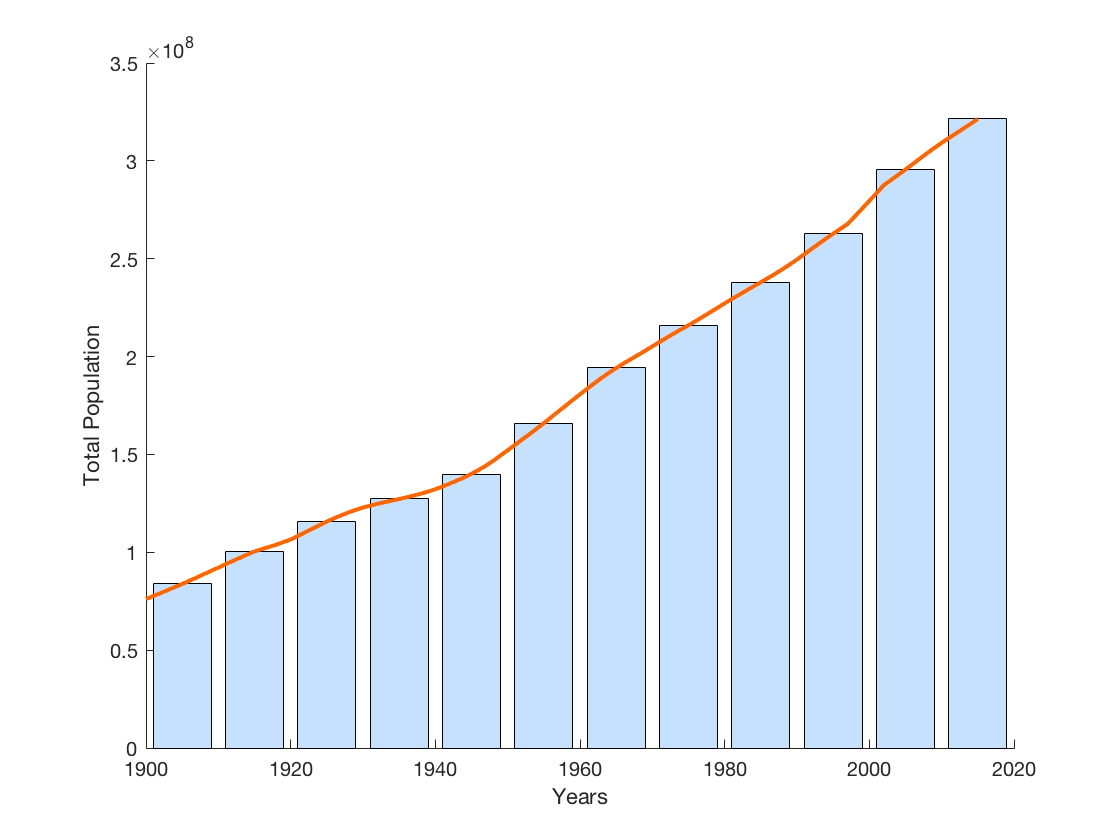
\includegraphics[width=0.7\textwidth,keepaspectratio]{images/us-population}
  \label{fig:us-population}
\end{figure}

\subsection{Clustered SELEIR Modell}

Das erste Modell ist das Clustered SELEIR Modell aus \cite{ModellingTBEpidemics2009} wie zu sehen in \ref{fig:clustered-seleir}.

\begin{figure}[ht]
  \centering
  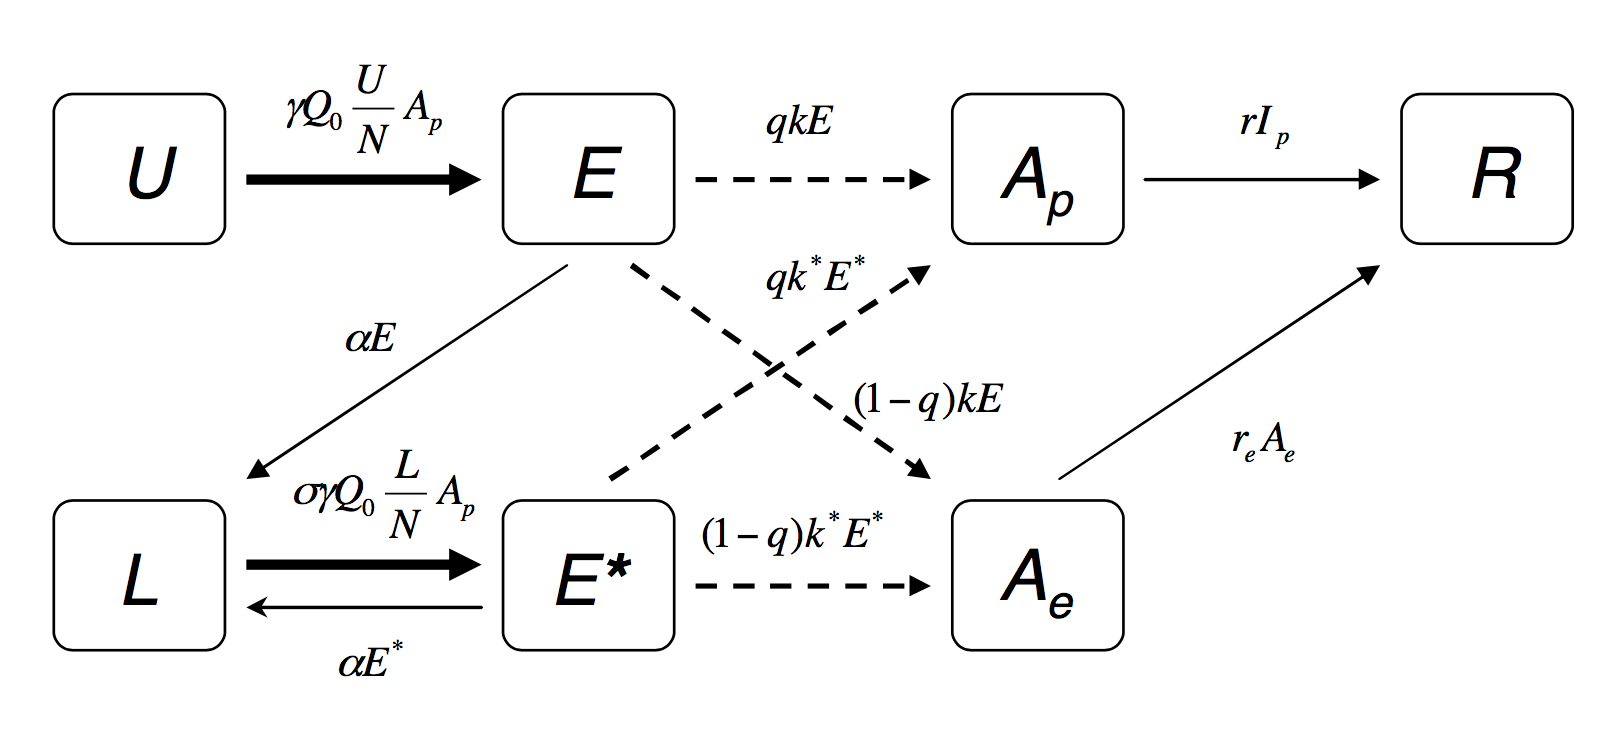
\includegraphics[width=0.9\textwidth,keepaspectratio]{images/clustered_seleir_model}
  \caption{Clustered Tuberkulose in \cite{ModellingTBEpidemics2009}}
  \label{fig:clustered-seleir}
\end{figure}

Das Transfer Diagramm zeigt einige Ähnlichkeiten zu den bisherigen Compartment Modellen nur deutlich komplexer. Um alles schwieriger zu machen sind $U$ die Empfänger ($S$), $A$ sind die infizierten ($I$) und $L$ ist eine neue Klasse von latent exposierten Individuen. Wie zuvor gillt der Kreislauf $U -> E -> A -> R$. Zusätzlich kommt hinzu das die latente Phase deutlich fein granularer dargestellt wird. Anstelle von dem direkten Übergang von latent infizierten $E$ zu infizierten gibt es drei Klassen. $E$ kann standardmäßig zur Klasse der Infizierten wandern. Hier gibt es zwei Klassen, der Befall der Lunge ``pulmonale TB'' $A$ oder der Befall anderer Organe ``extrapulmonale TB'' $A^{\*}$. $E$ kann außerdem in die Klasse $L$, lange latente Infizierte die eine wesentlich geringere Chance auf den Ausbruch haben. Diejenigen die $L$ mit einer Wahrscheinlichkeit $o\gamma Q_{0}\frac{L}{N}A_{p}$ verlassen sind in einer hochgradig exposierten Variante von $E$, die höhere Wahrscheinlichkeit auf aktiven Ausbruch hat. \\

Die Cluster Variante des obigen Systems kommt dadurch zustande das zwei Populationen durch zwei Differentialgleichungssysteme modelliert wird. Das obere System wird also dupliziert und eine explizite Abhängigkeit aufgebaut. Eine generelle Population $N_{1}$ bei der es zufällig mit einem sehr geringen Wert Neuinfektionen für TB gibt. Eine Population mit clustern von erkrankten $N_{2}$ die bei jeder Neuinfektion in $N_{1}$ dahin bewegt wird. Es gibt dann eine Kontaktwahrscheinlichkeit zwischen $N_{1}$ und $N_{2}$. Das volle Differentialgleichungssystem kann in \cite{ModellingTBEpidemics2009} nachvollzogen werden und würde den Rahmen hier sprengen.

\subsubsection{Experiment}

Das Experiment mit dem Clustered SELEIR Modell ist herauszufinden wie gut man mit generellen Populationsparametern für Tuberkulose die Kurve von realen Daten approximieren kann.

\blindtext

\subsection{Modell 2}

\blindtext

\subsubsection{Matlab}

\blindtext

\subsubsection{Resultate}

\blindtext

\section{Agentenbasierte Modellierung zur Ausbreitung von Tuberkulose}

\blindtext

\subsection{Modell}

\blindtext

\subsection{Mesa}

\blindtext

\subsection{Einfluss von Impfung}

\blindtext

\subsection{Einfluss von Immunerkrankungen}

\blindtext

\subsection{Einfluss von Lokalität}

\blindtext

\section{Statistische Modelle}

\blindtext

\section{Fazit}

In dieser Arbeit wurde gezeigt wie agentenbasierte Modellierung und Compartment Modelle genutzt werden können, um die Ausbreitung von Infektionskrankheiten wie Tuberkulose zu simulieren. Idealerweise kommen neue Erkenntnisse ans Licht, wie die Übertragung von Tuberkulose verhindert werden kann. Tuberkulose ist eine ernst zu nehmende Erkrankung der heutigen Zeit.

\newpage

\bibliographystyle{apalike}
\bibliography{md-tuberkulose}

\end{document}

